\documentclass{beamer}
\usetheme{Boadilla}  %Boadilla, Madrid
\usepackage[utf8]{inputenc}
%\usepackage[ansinew]{inputenc}
% \usepackage[german]{babel}  % noetig fuer Umlaute
\usepackage[english]{babel}
\usepackage{array}
\graphicspath{{Bildmaterial/}}
% \usepackage{wrapfig}
\usepackage{multimedia}
\usepackage{hyperref}
\usepackage{ulem}
\usepackage{color}
\usepackage{siunitx}
\usepackage{amssymb}
\beamertemplatenavigationsymbolsempty
\usepackage{multirow}
% \usepackage{dsfont} % for identity matrix \mathds{1}
%\newcommand{\RM}[1]{\MakeUppercase{\romannumeral #1{.}}}

%%% for Code Snipplets
\usepackage{listings}
\usepackage{color}

\definecolor{dkgreen}{rgb}{0,0.6,0}
\definecolor{gray}{rgb}{0.5,0.5,0.5}
\definecolor{mauve}{rgb}{0.58,0,0.82}

\lstset{
  language=[90]Fortran,
  aboveskip=3mm,
  belowskip=3mm,
  showstringspaces=false,
  columns=fullflexible,
  basicstyle={\small\ttfamily},
  numbers=none,
  numberstyle=\small\color{gray},
  keywordstyle=\color{mauve},
  commentstyle=\color{dkgreen},
  stringstyle=\color{blue},
  breaklines=true,
  breakatwhitespace=false,
  tabsize=3
}
%---------------------------------------------------------------------

%% how to include graphics
% \begin{figure}[H]
%   \centering
%   \includegraphics[width=1\textwidth]{}
%   \caption{}
%   \label{fig:...}
% \end{figure}

%---------------------------------------------------------------------
%---------------------------------------------------------------------
%---------------------------------------------------------------------

\title{grav\_project level 0}

\author{Philipp Denzel}
\date{\today}
\institute{Universität Zürich}
 
\begin{document}
\begin{frame}
 \LARGE
 \sf 	   grav\_project Level 0 \\ 
	   My Version of the Program \\

\rule{0.8\textwidth}{0.5pt} \\ % horizontal line of variable length and width
 \Large Denzel, Philipp \\
\rule{0.8\textwidth}{0.5pt} \\  % horizontal line of variable length and width
  \text{Email:} \\ phdenzel@hispeed.ch \\
\end{frame}
%---------------------------------------------------------------------
\begin{frame}
  \frametitle{Structure of First Program}
  
  \begin{itemize}
   \item Open files
   \item Read data into arrays
   \item Loop through all grid points (force)
   \item Nested loop through all grid centres (density)
   \item Calculate formula inside inner loop
   \item Write force into new file
  \end{itemize}

\end{frame} 
%---------------------------------------------------------------------
\begin{frame}[fragile]
  \frametitle{Read Files}
  \begin{lstlisting}
   open(unit=8, file='/path/to/r_project.data', status='old', action='read')
   ! read radii into 1-D array
    do i = 1, N_r
        read(8, '(e20.10)') r_i
        r(i) = r_i
    end do
    close(unit=8)
  \end{lstlisting}
  
  for r(N\_r), theta(N\_theta), sigma(N\_r,N\_theta), dr(N\_r), dtheta(N\_theta)
  
\end{frame}
%---------------------------------------------------------------------
\begin{frame}[fragile]
  \frametitle{Simple Implementation}
  \lstset{
    language=[90]Fortran,
    aboveskip=3mm,
    belowskip=3mm,
    showstringspaces=false,
    columns=fullflexible,
    basicstyle={\tiny\ttfamily},
    numbers=none,
    numberstyle=\small\color{gray},
    keywordstyle=\color{mauve},
    commentstyle=\color{dkgreen},
    stringstyle=\color{blue},
    breaklines=true,
    breakatwhitespace=false,
    tabsize=3
}
      
  \begin{lstlisting}
  
    ! write force components for every corner in grid
    do i = 1, N_r
        r_i = r(i)-.5*dr(i) ! shift r to the corners
        do j = 1, N_theta
            theta_j = theta(j)-.5*dtheta(j) ! shift theta to the corners
            ! sum up the forces onto the point (i, j)
            do iprime = 1, N_r
                do jprime = 1, N_theta
                    force_point = -sigma(iprime,jprime)*r(iprime)*dr(iprime)*dtheta(jprime)/(r_i**2+r(iprime)**2-2.*r_i*r(iprime)*cos(theta_j-theta(jprime)))**(1.5)
                    f_r = f_r + force_point * (r_i-r(iprime)*cos(theta_j-theta(jprime)))
                    f_theta = f_theta + force_point * r(iprime)*sin(theta_j-theta(jprime))
                end do
            end do
        write(11, '(e20.10)') f_r
        write(12, '(e20.10)') f_theta
        f_r = 0.
        f_theta = 0.
        end do
    end do
  \end{lstlisting}
\end{frame}
%---------------------------------------------------------------------
\begin{frame}
 \frametitle{Optimization Strategy}
 \begin{itemize}
  \item Shift operations to outer loops, if possible
  \item Better programming syntax
  \item Idea: find faster methods, e.g. invsqrt (see later)
 \end{itemize}

\end{frame}
%---------------------------------------------------------------------
\begin{frame}[fragile]
  \frametitle{Write cos/sin Lookup Tables}
  Dimensions of the lookup table adjusted to the angular difference:
  \begin{lstlisting}
   REAL(8), DIMENSION(1-N_theta:N_theta-1) :: cos_table, sin_table
   ! fill the sin/cos table
    do j = 1,N_theta
        theta_j = theta(j)-.5*dtheta(j)
        do jprime = 1,N_theta
            diff_theta = theta_j-theta(jprime)
            cos_table(j-jprime) = cos(diff_theta)
            sin_table(j-jprime) = sin(diff_theta)
        end do
    end do
  \end{lstlisting}

\end{frame}
%---------------------------------------------------------------------
\begin{frame}[fragile]
  \frametitle{Write Mass Lookup Tables}
  \begin{lstlisting}
   ! fill the mass table
    do iprime = 1, N_r
        r_iprime = r(iprime)*dr(iprime) ! multiply dr already here to save some operations
        do jprime = 1,N_theta
            mass(iprime,jprime) = -sigma(iprime,jprime)*r_iprime*dtheta(jprime)
        end do
    end do
  \end{lstlisting}
  
  will change for every timestep

\end{frame}
%---------------------------------------------------------------------
\begin{frame}[fragile]
 \frametitle{Current Version}
  \lstset{
    language=[90]Fortran,
    aboveskip=3mm,
    belowskip=3mm,
    showstringspaces=false,
    columns=fullflexible,
    basicstyle={\tiny\ttfamily},
    numbers=none,
    numberstyle=\small\color{gray},
    keywordstyle=\color{mauve},
    commentstyle=\color{dkgreen},
    stringstyle=\color{blue},
    breaklines=true,
    breakatwhitespace=false,
    tabsize=3
}
  Diffrence to the first version in capital letters:
  \begin{lstlisting}
   ! write force components for every corner in grid
    do i = 1, N_r
        r_i = r(i)-.5*dr(i) ! shift r to the corners
        R_I_SQUARED = R_I*R_I   ! better than calculating it in formula
        do j = 1, N_theta
            theta_j = theta(j)-.5*dtheta(j) ! shift theta to the corners
            ! sum up the forces on the point (i, j)
            do iprime = 1, N_r
                R_IPRIME = R(IPRIME)  ! slight performance improvement
                R_IPRIME_SQUARED = R_IPRIME*R_IPRIME   ! slight performance improvement
                do jprime = 1, N_theta
                    ! formula for the gravitational force split into four parts for faster calculation
                    R_IPRIME_COS = R_IPRIME*COS_TABLE(J-JPRIME)
                    DENOM_POINT = 1./SQRT(R_I_SQUARED+R_IPRIME_SQUARED-2.*R_I*R_IPRIME_COS)
                    DENOM_POINT = DENOM_POINT * DENOM_POINT * DENOM_POINT
                    force_point = MASS(IPRIME,JPRIME) * DENOM_POINT
                    f_r = f_r + force_point * (R_I-R_IPRIME_COS)
                    f_theta = f_theta + force_point * R_IPRIME*SIN_TABLE(J-JPRIME)
                end do
            end do
        write(11, '(e20.10)') f_r
        write(12, '(e20.10)') f_theta
        f_r = 0.
        f_theta = 0.
        end do
    end do
  \end{lstlisting}

\end{frame}
%---------------------------------------------------------------------
\begin{frame}
 \frametitle{InvSqrt}
 \url{http://en.wikipedia.org/wiki/Fast_inverse_square_root}
\end{frame}
%---------------------------------------------------------------------
\begin{frame}[fragile]
 \frametitle{Custom InvSqrt}
  \lstset{
    language=[90]Fortran,
    aboveskip=3mm,
    belowskip=3mm,
    showstringspaces=false,
    columns=fullflexible,
    basicstyle={\tiny\ttfamily},
    numbers=none,
    numberstyle=\small\color{gray},
    keywordstyle=\color{mauve},
    commentstyle=\color{dkgreen},
    stringstyle=\color{blue},
    breaklines=true,
    breakatwhitespace=false,
    tabsize=3
}
  \begin{lstlisting}
   REAL(8) FUNCTION InvSqrt (x)
    IMPLICIT NONE
    TYPE casting
        REAL(8) :: x
    END TYPE casting
    REAL(8), INTENT(in) :: x
    ! casting
    TYPE(casting), TARGET :: pointerTo
    ! Encode data as an array of integers
    INTEGER(8), DIMENSION(:), ALLOCATABLE :: enc
    INTEGER(8) :: length
    INTEGER(8) :: magic_number = 6910469410427058089
    REAL(8) :: xhalf
    xhalf = .5*x
    ! transfer to heap
    pointerTo%x = x
    ! encode a memory section from a type to other
    length = size(transfer(pointerTo, enc))
    allocate(enc(length))
    ! encoded to integer
    enc = transfer(pointerTo, enc)  ! evil floating point bit level hacking
    enc(1) = magic_number - rshift(enc(1),1)  ! wtf! (for int64: 0x5fe6eb50c7b537a9 = 6910469410427058089)
    ! decode
    pointerTo = transfer(enc, pointerTo)
    ! dealloc
    deallocate(enc)

    InvSqrt = pointerTo%x*(1.5 - xhalf*pointerTo%x*pointerTo%x)
END FUNCTION InvSqrt
  \end{lstlisting}

\end{frame}
%---------------------------------------------------------------------
\begin{frame}
 \frametitle{Alternative}
  Intel Programming Environment: SSE instructions rsqrtss/rsqrtps
\end{frame}
%---------------------------------------------------------------------
\begin{frame}
 \begin{figure}[H]
  \centering
  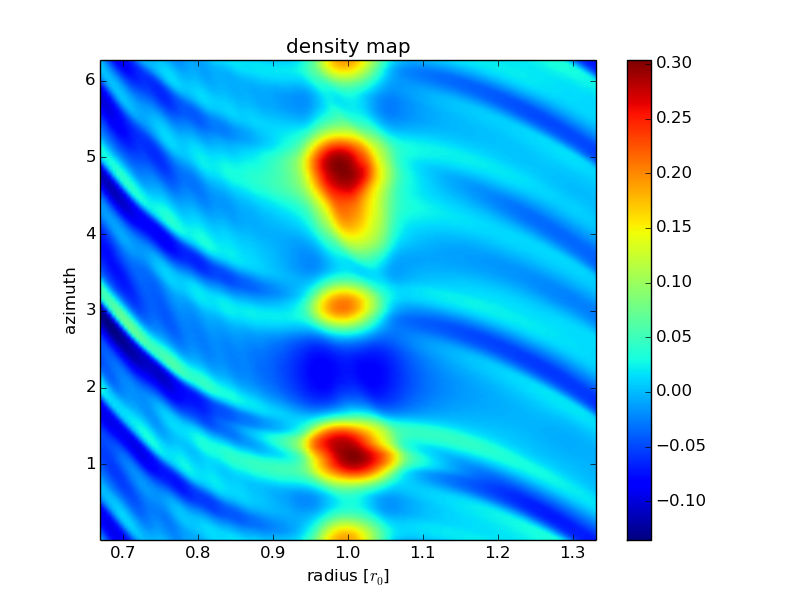
\includegraphics[width=1\textwidth]{density.png}
\end{figure}
\end{frame}
%---------------------------------------------------------------------
\begin{frame}
 \begin{figure}[H]
  \centering
  \includegraphics[width=1\textwidth]{radial_force_orig.png}
\end{figure}
\end{frame}
%---------------------------------------------------------------------
\begin{frame}
 \begin{figure}[H]
  \centering
  \includegraphics[width=1\textwidth]{angular_force_orig.png}
\end{figure}
\end{frame}
%---------------------------------------------------------------------
\begin{frame}[fragile]
  \frametitle{Timings}
  {\tiny
  \begin{verbatim}
------------------------------------------------------------------------------------------------------------
 OPTIMAL TIME STANDS AT:   10.2038803 sec -> current standard

 without mass array    255.950150
                                   (slight performance improvements by avoiding too many array calls)
    with mass array    152.530518
                                   (half mass calc operations; inner loop)
sin/cos inside loop    119.338303
                                   (one cos calculation eliminated; inner loop)
   with denominator    57.8149910
                                   (denominator using sqrt*sqrt*sqrt instead **1.5)
with sin/cos tables    17.7189388
                                   (calculating cos/sin in external loop)
         mass table    15.7216377
                                   (calculating the mass in external loop)
  with r_iprime_cos    14.8603277
                                   (saves a few calculations in the inner loop since it appears twice there)
 optimizer flag -O1    10.2038803
                                   (remembered that gnu compilers have no optimization default)
     custom invsqrt    84.1394730
                                   (sadly much slower than intrinsic 1./sqrt,
                                         but the error is actually not that bad)
------------------------------------------------------------------------------------------------------------
  \end{verbatim}}
\end{frame}
\end{document}